\chapter{Phase shift transducer}
\section{Theory and related work} \label{sec:literature_phase}
A phase shift transducer converts the phase shift between two signals to an analog DC output.  For the purpose of this project, an XOR-gate based phase detector is used to implement this transducer. The presence of a phase shift between two signals introduces an equivalent time delay between them. An XOR gate produces a logical high when its two inputs have different logical states, which would occur during this time delay. The resultant output is a square signal with a duty cycle equal to the time shift between the two original signals. Thus, the width of the pulse of the output signal changes proportionally to the phase difference between the input signals and is said to be pulse-width modulated (PWM)\cite{phase_detector}. The XOR phase detector can only be used for phase shifts of $\numrange{0^o}{180^o}$, thus, it is sufficient for this project.

Since the input signals (voltage and current) are sinusoidally varying, they must be modified before being supplied to the XOR gate. To obtain the required digital signals, a comparator can be used. By having the same reference for both comparators, the XOR inputs will be offset by the same time delay as the sinusoidal signals as required. 

However, the XOR phase detector outputs a digital signal. To convert this to an analog value, a demodulator for the PWM signal must be considered. The simplest of these is a low pass RC filter\cite{pwm_low_pass}. By setting the RC constant to be much larger than the PWM signal period, the filter acts as an integrator. Its output is then the average of the XOR gate output signal. The behaviour of the phase transducer can thus be described as: $V_{out} = V_{DD} \times \frac{\Delta\Theta}{180^o}$\cite{phase_detector}

Since the range of the phase detector is up to $180^o$, the resolution may be impacted. To improve this an amplification stage is added to map $45^o$ closer to the maximum range. While this would cause clipping for higher phase shifts, it is not a major concern given this project's specifications. A standard non-inverting amplifier, as shown in Figure \ref{fig:non_invert_amp} can be used for this.

\section{Design} \label{sec:design_phase}
The design of the transducer begins with the two comparators for the voltage and input signals. The TLC2272 op-amps are chosen for this, as they produce sufficiently high voltage, so as to be seen as a logical high by an XOR gate\cite{XOR}. The reference for both is also chosen to be $\SI{0}{\volt}$ as it is easily obtained by connecting to the ground plane. The voltage signal to the comparator must first be scaled down to be within the common-mode and input voltage limits of the op-amp. Equation \ref{eqn:voltage_divider} shows the ratio of the voltage divider to be used for this purpose. The same voltage divider is used for the input of the voltage comparator as it complies with the common-mode, differential and input limits as shown in Section \ref{sec:design_voltage}. 

For the current signal comparator, it is considered that the current sense resistor provides extremely low voltages.Some of these are even less than the op-amp's input offset voltage and would therefore affect the comparator's performance. A non-inverting amplifier is therefore designed to amplify the signal to a more usable range. An amplifier for the current signal had been designed in Section \ref{sec:design_current}, but combined with a precision rectifier. Isolating just the amplifier gives a signal that should conform  to the limits(common-mode, differential and input voltages) of the op-amp used for the comparator as previously shown. 

It is however observed during simulation, that the non-inverting amplifier introduces a small DC offset, such that the amplified signal is no longer centred around $\SI{0}{\volt}$. So, the current comparator setup would not provide the required output. To counteract this, the amplified signal is measured and found to be centred around $\SI{54}{\milli\volt}$. The inverting input of the op-amp is thus connected to a voltage approximately equal to this by passing the +5V supply through a voltage divider circuit. Selecting a $\SI{100}{\kilo\ohm}$ and $\SI{1}{\kilo\ohm}$ resistor gives: $V_{ref} = \frac{1\si{\kilo}}{1\si{\kilo}+100\si{\kilo}} \times 5 = \SI{49.5}{\milli\volt}$. As this value may vary from op-amp to op-amp, a $\SI{1}{\kilo\ohm}$ potentiometer is chosen for the final design, so that it can be manually tuned in practice.

As the XOR gate can only handle voltages greater than $\SI{-0.5}{\volt}$ at its input\cite{XOR}, the outputs of the comparator are passed through a diode before the gate. The XOR gate is then supplied with the previously designed $\SI{+5}{\volt}$ supply.

As explained before, the RC filter must have a RC constant much larger than the PWM signal period. This also has the upside of reducing the ripple voltage at its output. However, making this constant too large increases the settling time of the filter, thus, a balance between the two must be achieved. Selecting a $\SI{1}{\mu\farad}$ capacitor, the resistor can be calculated to be: $RC > 10 \times T = 0.1$. Thus the resistor should be larger than $\SI{100}{\kilo\ohm}$. A $\SI{470}{\kilo\ohm}$ potentiometer is used in this place and tuned accordingly in practice, so as to balance the above mentioned trade-off.


For the maximum specification of $45^o$, the phase detector gives an output of 1.25V. The gain of the non-inverting amplifier is chosen such that this is mapped to 4.5V, which is sufficiently close to the rails. This gives a gain of 3.6. Choosing resistors as $\SI{5.6}{\kilo\ohm}$ and $\SI{2.2}{\kilo\ohm}$ gives: $1+\frac{4.7k}{2.2k} = 2.14$.

As a 10-bit ADC is to be used, the resolution is given as 4.883mV/bit. Reversing this to the input of the transducer gives a resolution of $\SI{6.227}{\mu}$s/bit or $0.1121^o$/bit.

The complete phase shift transducer circuit is given in Figure \ref{fig:phase_circuit}.

\begin{figure}
        \centering
         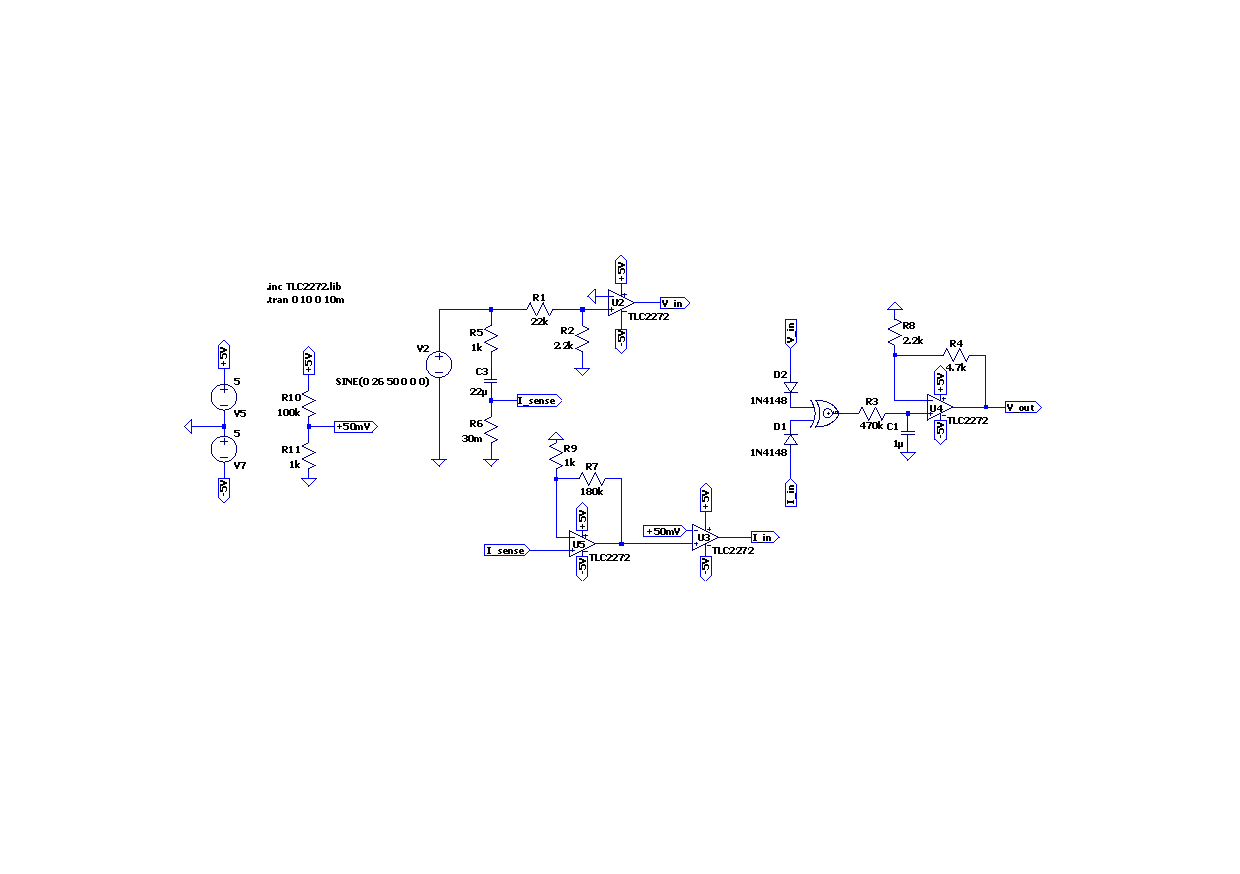
\includegraphics[width=1.15\linewidth,clip, trim = 3cm 3cm 0cm 3cm]{./Figures/phase_circuit.pdf}
		    \caption{Phase shift transducer circuit.} \label{fig:phase_circuit}
 \end{figure}

\section{Simulation} \label{sec:simulation_phase}

\begin{figure}[h] 
 \centering
 
    \begin{subfigure}[]{0.65\linewidth}
        \centering
        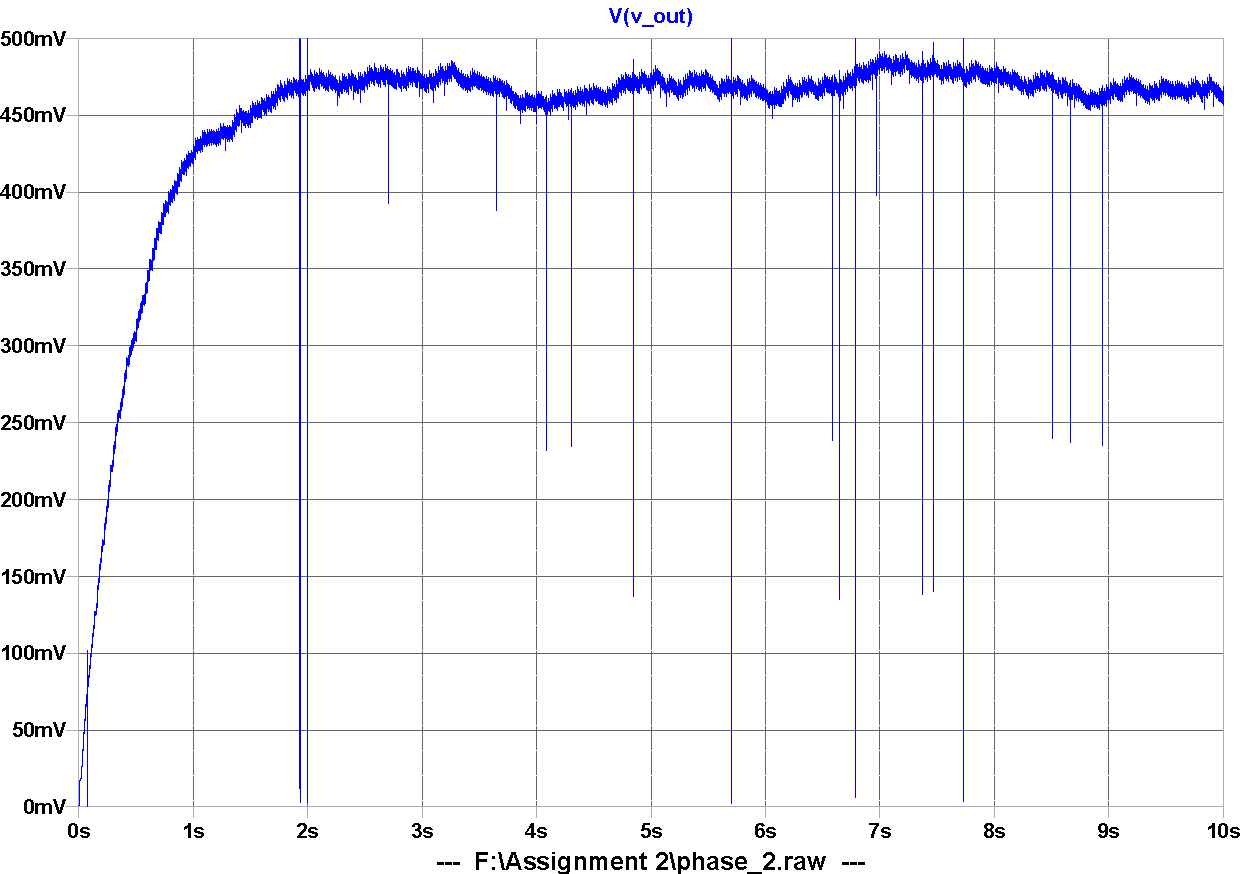
\includegraphics[width=1.\linewidth]{./Figures/phase_transducer_simulation_22u.pdf}
        \caption{$\SI{1}{\kilo\ohm}$ and $\SI{22}{\mu\farad}$ load.}
        \label{fig:phase_simulation_22u}
    \end{subfigure}
    \begin{subfigure}[]{0.65\linewidth}
        \centering
        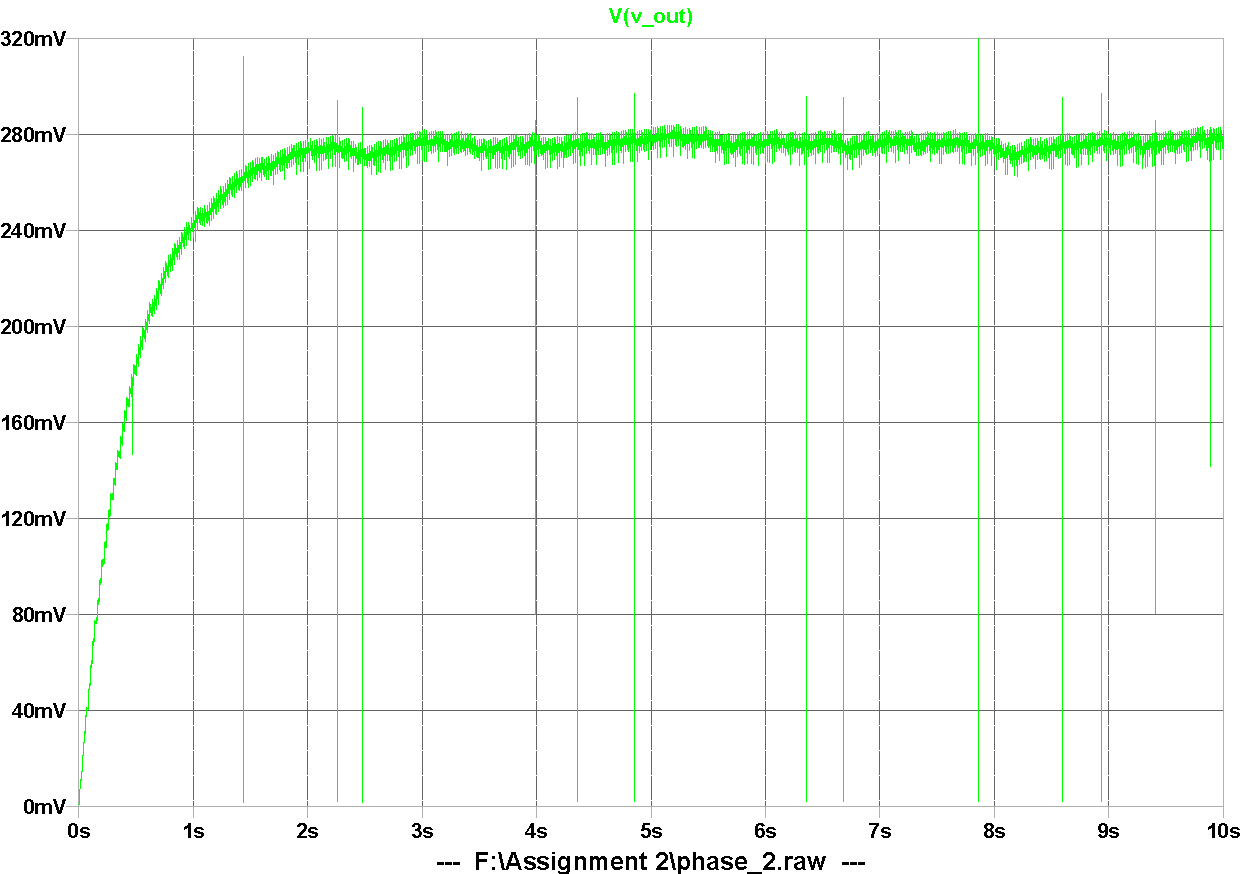
\includegraphics[width=1.\linewidth]{./Figures/phase_transducer_simulation_33u.pdf}
        \caption{$\SI{1}{\kilo\ohm}$ and $\SI{33}{\mu\farad}$ load.}
	    \label{fig:phase_simulation_33u}
    \end{subfigure}
    
\caption{Phase shift transducer simulation for nominal loads.}
\end{figure}

\section{Measurements} \label{sec:measurements_phase}
The conversion in Table \ref{tab:phase_integrated_test} is derived from the circuit in Figure \ref{fig:phase_circuit}.

$V_{out} = (1 + \frac{4.7k}{2.2k}) \times 5 \times \frac{\Delta\Theta}{180^o} = \Delta\Theta(0.08712)$
\begin{figure}
 \centering
     \begin{subfigure}[]{0.45\textwidth}
        \centering
         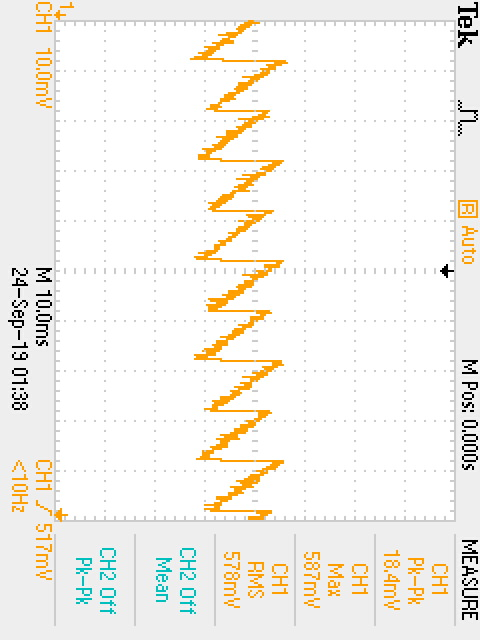
\includegraphics[height=1\linewidth,angle =90]{./Figures/phase_measure}
		    \caption{AC input and DC output for mid range load.} \label{subfig:phase_measure}
     \end{subfigure}
      \begin{subfigure}[]{0.45\textwidth}
              \centering
  		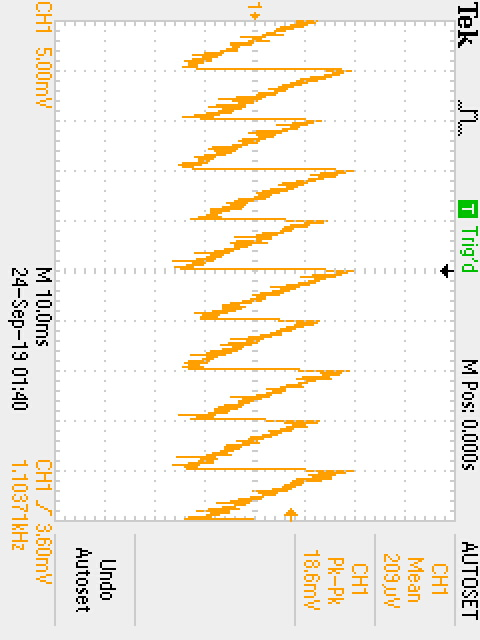
\includegraphics[height=1\linewidth,angle=90]{./Figures/phase_noise_measure}
		    \caption{Voltage transducer noise levels for a mid sized load.} \label{subfig:phase_noise}
     \end{subfigure}
 \end{figure}

\begin{table}[h]
        \centering
        \footnotesize
        \caption{Phase shift transducer unit test results}
         \begin{tabular}{p{1.8cm}p{1.3cm}p{1.3cm}p{1.5cm}p{1.5cm}p{1.8cm}p{1.8cm}p{1.8cm}}
          \toprule
             \textit{\footnotesize Measurement} & \textit{\footnotesize Load R} & \textit{\footnotesize Load C} & \textit{{\footnotesize Measured shift}} & \textit{{\footnotesize Applied shift}} & \textit{{\footnotesize Analogue output}} & \textit{\footnotesize Conversion} & \textit{\footnotesize Difference}\\
             & $[\si{\ohm}]$ & $[\si{\mu\farad}]$ & $[ms]$ & $[^o]$ & $[\si{\volt}DC]$ & $[^o]$ & $[^o]$ \\
          \midrule
          No phase shift & 1k & none & 0.036 & 0.648 & 0.173 & 1.986 & 1.338 \\
          Max phase shift & 1k & 3.3 & 1.92 & 34.56 & 2.834 & 32.53 & 2.03 \\
          Mid range & 1k & 22 & 0.458 & 8.244 & 0.608 & 6.9788 & 1.265 \\
          Mid + $\delta$ & 1k & 33 & 0.286 & 5.148 & 0.335 & 3.845 & 1.303 \\
          Mid + $2\delta$ & 1k & 47 & 0.196 & 3.528 & 0.1806 & 2.073 & 1.455 \\
          \bottomrule
        \end{tabular}
     \label{tab:phase_integrated_test}
\end{table}







